\chapter{Sistemi di Tempo nella Meccanica Celeste}
\label{ch:time_systems}

La misurazione del tempo è fondamentale per la meccanica celeste, ma sorprendentemente complessa. Diverse applicazioni richiedono diverse scale temporali, ciascuna con definizioni e casi d'uso specifici. Questo capitolo descrive i sistemi temporali implementati in AstDyn e le loro interconversioni.

\section{Perché Sistemi Temporali Multipli?}

Un approccio ingenuo potrebbe usare il tempo civile ordinario (UTC) per tutti i calcoli. Tuttavia, questo è inadeguato per la meccanica celeste di precisione a causa di:

\begin{itemize}
    \item \textbf{Rotazione irregolare della Terra}: La lunghezza di un giorno varia a causa dell'attrito mareale, effetti atmosferici e accoppiamento nucleo-mantello
    \item \textbf{Secondi intercalari}: UTC include salti discontinui per rimanere sincronizzato con la rotazione terrestre
    \item \textbf{Effetti relativistici}: Il tempo scorre diversamente in diversi potenziali gravitazionali
    \item \textbf{Requisiti di precisione}: Accuratezza sub-secondo su secoli richiede un cronometraggio accurato
\end{itemize}

\section{Numero di Giorno Giuliano}

Prima di discutere le scale temporali specifiche, introduciamo il sistema del Giorno Giuliano (JD), un conteggio continuo di giorni dal mezzogiorno UTC del 1 gennaio 4713 a.C. (calendario giuliano prolettico).

\begin{definition}[Giorno Giuliano]
Il Numero di Giorno Giuliano (JD) è il numero di giorni trascorsi dall'epoca JD 0.0 = 12:00 UT del 1 gennaio 4713 a.C.
\end{definition}

Per esempio:
\begin{itemize}
    \item 1 gennaio 2000, 12:00 TT = JD 2451545.0
    \item 26 novembre 2025, 00:00 UTC $\approx$ JD 2460638.5
\end{itemize}

\subsection{Giorno Giuliano Modificato}

Per ridurre i requisiti di precisione numerica, il \textit{Giorno Giuliano Modificato} (MJD) è comunemente usato:

\begin{equation}
\text{MJD} = \text{JD} - 2400000.5
\end{equation}

Questo sposta l'epoca al 17 novembre 1858, 00:00 UTC, e inizia i giorni a mezzanotte anziché a mezzogiorno. L'epoca di riferimento J2000.0 corrisponde a:

\begin{equation}
\text{MJD}_{\text{J2000}} = 51544.5
\end{equation}

AstDyn usa principalmente MJD per i calcoli interni.

\section{Tempo Universale (UT)}

Il Tempo Universale (UT) è basato sulla rotazione terrestre. Esistono diverse varianti:

\subsection{UT0}

UT0 è il Tempo Universale grezzo come misurato osservando le posizioni stellari. Varia a causa del movimento polare (oscillazione dell'asse di rotazione terrestre).

\subsection{UT1}

UT1 corregge UT0 per gli effetti del movimento polare:

\begin{equation}
\text{UT1} = \text{UT0} + \Delta \lambda
\end{equation}

dove $\Delta\lambda$ tiene conto dello spostamento della longitudine dell'osservatore dovuto al movimento polare. UT1 rappresenta il vero angolo rotazionale della Terra.

\subsection{UTC (Tempo Universale Coordinato)}

UTC è lo standard del tempo civile, definito da orologi atomici ma mantenuto entro 0.9 secondi da UT1 inserendo \textit{secondi intercalari}. La differenza è:

\begin{equation}
\Delta UT = \text{UT1} - \text{UTC}
\end{equation}

I secondi intercalari sono annunciati dal Servizio Internazionale di Rotazione Terrestre (IERS) e tipicamente occorrono il 30 giugno o il 31 dicembre.

\begin{figure}[H]
\centering
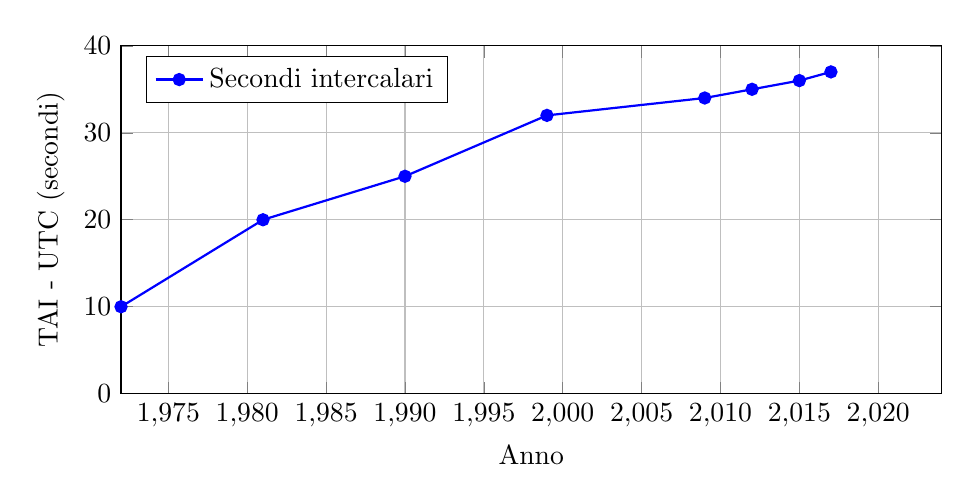
\begin{tikzpicture}
    \begin{axis}[
        width=12cm,
        height=6cm,
        xlabel={Anno},
        ylabel={TAI - UTC (secondi)},
        xmin=1972,
        xmax=2024,
        ymin=0,
        ymax=40,
        grid=major,
        legend pos=north west
    ]
    \addplot[blue, thick, mark=*] coordinates {
        (1972,10) (1981,20) (1990,25) (1999,32)
        (2009,34) (2012,35) (2015,36) (2017,37)
    };
    \legend{Secondi intercalari}
    \end{axis}
\end{tikzpicture}
\caption{Accumulo di secondi intercalari dal 1972}
\label{fig:leapseconds}
\end{figure}

\section{Scale di Tempo Atomiche}

\subsection{TAI (Tempo Atomico Internazionale)}

TAI è una scala temporale continua e uniforme definita da un insieme di orologi atomici in tutto il mondo. Non ha secondi intercalari e forma la base per altre scale temporali moderne.

La relazione con UTC è:

\begin{equation}
\text{TAI} = \text{UTC} + \Delta AT
\end{equation}

dove $\Delta AT$ è il numero cumulativo di secondi intercalari (37 secondi a partire dal 2024).

\subsection{TT (Tempo Terrestre)}

Il Tempo Terrestre è la scala temporale teorica per osservazioni sulla superficie terrestre. È correlato a TAI da un offset costante:

\begin{equation}
\text{TT} = \text{TAI} + 32.184 \text{ s}
\end{equation}

L'offset di 32.184 secondi è stato scelto per mantenere la continuità con la vecchia scala di Tempo delle Effemeridi (ET). TT è l'argomento temporale per le effemeridi geocentriche.

\subsection{TDB (Tempo Dinamico Baricentrico)}

Il Tempo Dinamico Baricentrico è la scala temporale per i calcoli al baricentro del sistema solare (centro di massa). A causa degli effetti relativistici generali, il tempo scorre a velocità diverse in diversi potenziali gravitazionali.

La relazione tra TDB e TT include termini sia periodici che secolari:

\begin{equation}
\text{TDB} = \text{TT} + 0.001658 \sin(g) + 0.000014 \sin(2g) \text{ secondi}
\end{equation}

dove $g$ è l'anomalia media dell'orbita terrestre attorno al Sole:

\begin{equation}
g = 357.53° + 0.9856003°(JD - 2451545.0)
\end{equation}

Questa correzione è tipicamente di pochi millisecondi ma si accumula su lunghi periodi di tempo.

\section{Relazioni tra Scale Temporali}

La Figura~\ref{fig:timescales} illustra le relazioni tra le scale temporali:

\begin{figure}[H]
\centering
\begin{tikzpicture}[
    node distance=2.5cm,
    box/.style={rectangle, draw, fill=blue!10, text width=2cm, align=center, minimum height=1cm},
    arrow/.style={->, >=stealth, thick}
]
    \node[box] (utc) {UTC};
    \node[box, right=of utc] (tai) {TAI};
    \node[box, right=of tai] (tt) {TT};
    \node[box, right=of tt] (tdb) {TDB};
    \node[box, below=of utc] (ut1) {UT1};
    
    \draw[arrow] (utc) -- node[above] {\small $+\Delta AT$} (tai);
    \draw[arrow] (tai) -- node[above] {\small $+32.184$ s} (tt);
    \draw[arrow] (tt) -- node[above] {\small $+\Delta T_{rel}$} (tdb);
    \draw[arrow] (utc) -- node[left] {\small $+\Delta UT$} (ut1);
\end{tikzpicture}
\caption{Relazioni tra le principali scale temporali}
\label{fig:timescales}
\end{figure}

\section{Implementazione in AstDyn}

La classe \texttt{TimeScale} gestisce le conversioni tra i sistemi temporali:

\begin{lstlisting}[style=cpp,caption={Conversioni di scale temporali}]
#include <astdyn/time/TimeScale.hpp>
using namespace astdyn::time;

// Conversione UTC a TDB
double mjd_utc = 61000.0;
double mjd_tdb = TimeScale::utc_to_tdb(mjd_utc);

// TT a TAI
double mjd_tt = 61000.0;
double mjd_tai = TimeScale::tt_to_tai(mjd_tt);

// UT1 a UTC (richiede Delta_UT da IERS)
double delta_ut = 0.15;  // secondi, da IERS Bulletin A
double mjd_ut1 = 61000.0;
double mjd_utc_computed = mjd_ut1 - delta_ut / 86400.0;
\end{lstlisting}

\subsection{Tabella dei Secondi Intercalari}

AstDyn mantiene una tabella interna di secondi intercalari, aggiornata periodicamente:

\begin{table}[H]
\centering
\caption{Secondi intercalari recenti (tabella parziale)}
\label{tab:leapseconds}
\begin{tabular}{@{}lcc@{}}
\toprule
\textbf{Data} & \textbf{MJD} & \textbf{TAI-UTC (s)} \\
\midrule
2012-07-01 & 56109 & 35 \\
2015-07-01 & 57204 & 36 \\
2017-01-01 & 57754 & 37 \\
\bottomrule
\end{tabular}
\end{table}

\subsection{Approssimazioni di $\Delta T$}

Per date storiche o previsioni future dove i secondi intercalari sono sconosciuti, formule empiriche approssimano $\Delta T = \text{TT} - \text{UT}$:

\textbf{Prima del 1972} (adattamento polinomiale):
\begin{equation}
\Delta T \approx -20 + 32t^2 \text{ secondi}
\end{equation}
dove $t$ è in secoli dal 1820.

\textbf{Dopo il 2015} (estrapolazione lineare):
\begin{equation}
\Delta T \approx 69.2 + 0.4 \times (y - 2015) \text{ secondi}
\end{equation}
dove $y$ è l'anno.

Queste approssimazioni hanno incertezze di diversi secondi e non dovrebbero essere usate per lavoro preciso.

\section{Considerazioni Pratiche}

\subsection{Quale Scala Temporale Usare?}

\begin{description}
    \item[Osservazioni] Usare UTC per registrare i tempi di osservazione (facilmente sincronizzabile con GPS)
    \item[Calcoli orbitali] Convertire in TDB per l'integrazione numerica
    \item[Rotazione terrestre] Usare UT1 per calcolare il tempo siderale e le coordinate topocentriche
    \item[Reporting] Usare UTC per disseminare risultati agli osservatori
\end{description}

\subsection{Requisiti di Precisione}

Per la tipica determinazione di orbite asteroidali:
\begin{itemize}
    \item Accuratezza posizionale: $\sim 0.1''$ (arcosecondo)
    \item Accuratezza temporale necessaria: $\sim 0.01$ s
    \item Effetto di 1 secondo di errore temporale: $\sim 15''$ in AR per asteroide della fascia principale
\end{itemize}

Pertanto, usare la scala temporale corretta e tenere conto dei secondi intercalari è essenziale.

\subsection{Esempio: Catena di Conversione Temporale}

Conversione completa da data civile a TDB:

\begin{lstlisting}[style=cpp,caption={Conversione di data calendario a TDB}]
// Input: data civile UTC
int year = 2025, month = 11, day = 26;
double hour = 12.5;  // 12:30 UT

// Passo 1: Calendario a Giorno Giuliano
double jd_utc = calendar_to_jd(year, month, day + hour/24.0);
double mjd_utc = jd_utc - 2400000.5;

// Passo 2: UTC a TDB
double mjd_tdb = TimeScale::utc_to_tdb(mjd_utc);

std::cout << "MJD (TDB): " << std::fixed << std::setprecision(6) 
          << mjd_tdb << std::endl;
// Output: MJD (TDB): 61000.520833
\end{lstlisting}

\section{Letture Approfondite}

Le specifiche dettagliate dei sistemi temporali sono mantenute da:
\begin{itemize}
    \item \textbf{IERS} (International Earth Rotation Service): \url{https://www.iers.org}
    \item \textbf{BIPM} (Bureau International des Poids et Mesures): Definizione TAI
    \item \textbf{IAU} (International Astronomical Union): Risoluzioni sulle scale temporali
    \item \textbf{USNO} (US Naval Observatory): \textit{Astronomical Almanac}
\end{itemize}

La libreria SOFA (Standards of Fundamental Astronomy) fornisce implementazioni di riferimento delle trasformazioni temporali e di coordinate: \url{http://www.iausofa.org}